\section{More Complex Formulas}
The formulas in the previous section are common formulas, but are fairly simple. The benefit of using temporal logics is that a wide variety of behaviours can be expressed, including propositions about the robot \textit{and} about the workspace. Up to now, we have not looked at any formulas that include atomic propositions about potential tasks. We will show through examples that the same ideas presented in the previous chapter still hold true for this complex tasks, and show the speed up we get by using our algorithm compared to the accepted algorithm. 

\subsection{Example 1}
We look at the example from \cite{guo15} which says "eventually pick up the red ball. Once it is done, move to one basket and drop it. At last come back to room one and stay there". This task can be written as the LTL formula $\varphi = \diamond (\text{pickrball} \wedge \diamond \text{droprball}) \wedge \diamond \square r1$. The B\"uchi automaton corresponding to this formula as translated by \cite{gastin01} is shown in figure \ref{fig:buchiEx1}, with pick being short for pickrball and drop being short for droprball.

\begin{figure*}[!htb]
\centering
\includegraphics[scale=0.4]{buchiEx1_1}
\caption{B\"uchi Automaton Corresponding to $\varphi = \diamond (\text{pickrball} \wedge \diamond \text{droprball}) \wedge \diamond \square r1$}
\label{fig:buchiEx1}
\end{figure*} 

As we can see, there are many edges in this automaton and edges that have \&\& in the label. These paths can only be taken if we satisfy both of the propositions at the same time. However, because in our example the propositions do not overlap (the ball is not in the same room as the basket, and the neither the ball or basket is located in room 1) these edge are impossible to take. Therefore we remove these edges from the automaton (show the code for this). We then have a much simpler automaton that is shown in figure \ref{fig:ex1SimplifiedBuchi}

\begin{figure}
\centering
\begin{tikzpicture}[->,>=stealth',shorten >=1pt,auto,node distance=2.8cm,
                    semithick]
  \tikzstyle{every state}=[fill=red,draw=black,text=black]

  \node[initial,state] (A)                    {$q_1$};
  \node[state] (B)                    [right of=A]{$q_2$};
  \node[state] (C)                    [right of=B]{$q_4$};
  \node[state] (E)                    [above of=B]{$q_3$};
  \node[state] (F)                    [above of=C]{$q_5$};
  \node[state,accepting]         (D) [right of=C] {$q_6$};

  \path (A) edge              node {pickrball} (B)
  		%(A) edge [loop above] node {$\neg \pi_1$} (A)
  		(B) edge [loop below] node {$\neg$ droprball} (B)
  		(B) edge              node {droprball} (C)
  		(A) edge              node {$\neg$pickrball} (E)
  		(E) edge              node {pickrball} (F)
  		(F) edge              node {droprball} (C)
  		(C) edge [loop below] node {$\neg r1$} (C)
  		(C) edge              node {$r1$} (D)
  		(E) edge [loop above] node {$\neg$pickrball} (E)
  		(F) edge [loop above] node {$\neg$droprball} (F)
  		(D) edge [loop above] node {$r1$} (D);
\end{tikzpicture}
\caption{Simplified B\"uchi Automaton for $\varphi = \diamond (\text{pickrball} \wedge \diamond \text{droprball}) \wedge \diamond \square r1$ 1}
\label{fig:ex1SimplifiedBuchi}
\end{figure} 

In this automaton, we can see that $d(q_1)=3$, $d(q_2)=2$, $d(q_3)=3$, $d(q_4)=1$, $d(q_5)=2$, $d(q_6)=0$. For the first time, we have a node that connects to the initial node which is on the same level as the initial node. Examining our algorithm, we see that we will not start a new Dijkstra search until we find a node which is a level bellow our current level. Therefore we will not start a new search until we find a node in the product automaton with projection onto $q_2$ or $q_5$.

We can also see that from the illustration of the workspace, that the ball (rball) is not located next to the initial node, so the first proposition must be $\neg$pickrball. Examining the automaton in figure \ref{fig:ex1SimplifiedBuchi} that then we are guaranteed to take a path through nodes with projection $q_3$ and that we will never go to a node with the projection of $q_2$. Therefore we are in the same situation as for sequencing i.e.\ there is only one sequence of actions that will satisfy the formula, implying that our algorithm will find the same path as the accepted algorithm, just faster. 

\begin{figure}[!htb]
\centering
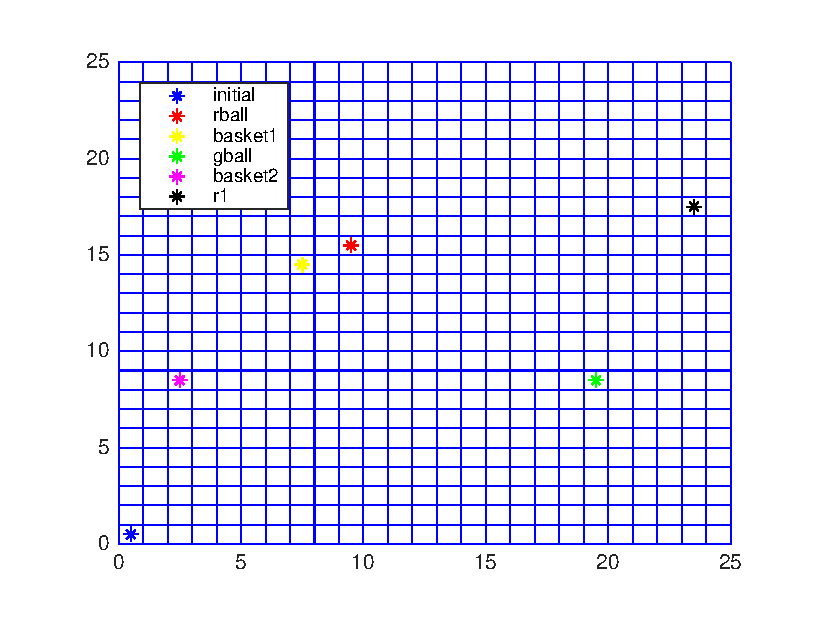
\includegraphics[scale=1]{workspace2.eps}
\label{fig:workspace2}
\end{figure}

We see that this is true in the output of the algorithms. Both give the same sequence of states and actions
\begin{lstlisting}
------------------------------
the prefix of plan **states**:
[((0, 0, 1), 'None'), ((0, 1, 1), 'None'), ((0, 2, 1), 'None'), ((1, 2, 1), 'None'), ((1, 3, 1), 'None'), ((2, 3, 1), 'None'), ((2, 4, 1), 'None'), ((3, 4, 1), 'None'), ((4, 4, 1), 'None'), ((4, 5, 1), 'None'), ((5, 5, 1), 'None'), ((5, 6, 1), 'None'), ((5, 7, 1), 'None'), ((6, 7, 1), 'None'), ((6, 8, 1), 'None'), ((7, 8, 1), 'None'), ((8, 8, 1), 'None'), ((8, 9, 1), 'None'), ((9, 9, 1), 'None'), ((9, 10, 1), 'None'), ((9, 11, 1), 'None'), ((9, 12, 1), 'None'), ((9, 13, 1), 'None'), ((9, 14, 1), 'None'), ((9, 15, 1), 'None'), ((9, 15, 1), 'pickrball'), ((9, 14, 1), 'None'), ((8, 14, 1), 'None'), ((7, 14, 1), 'None'), ((7, 14, 1), 'droprball'), ((7, 15, 1), 'None'), ((7, 16, 1), 'None'), ((7, 17, 1), 'None'), ((8, 17, 1), 'None'), ((9, 17, 1), 'None'), ((10, 17, 1), 'None'), ((11, 17, 1), 'None'), ((12, 17, 1), 'None'), ((13, 17, 1), 'None'), ((14, 17, 1), 'None'), ((15, 17, 1), 'None'), ((16, 17, 1), 'None'), ((17, 17, 1), 'None'), ((18, 17, 1), 'None'), ((19, 17, 1), 'None'), ((20, 17, 1), 'None'), ((21, 17, 1), 'None'), ((22, 17, 1), 'None'), ((23, 17, 1), 'None'), ((23, 17, 1), 'None')]
the suffix of plan **states**:
[((23, 17, 1), 'None'), ((23, 17, 1), 'None')]
------------------------------
the prefix of plan **actions**:
[(0, 0, 1), (0, 1, 1), (0, 2, 1), (1, 2, 1), (1, 3, 1), (2, 3, 1), (2, 4, 1), (3, 4, 1), (4, 4, 1), (4, 5, 1), (5, 5, 1), (5, 6, 1), (5, 7, 1), (6, 7, 1), (6, 8, 1), (7, 8, 1), (8, 8, 1), (8, 9, 1), (9, 9, 1), (9, 10, 1), (9, 11, 1), (9, 12, 1), (9, 13, 1), (9, 14, 1), (9, 15, 1), 'pickrball', (9, 14, 1), (8, 14, 1), (7, 14, 1), 'droprball', (7, 15, 1), (7, 16, 1), (7, 17, 1), (8, 17, 1), (9, 17, 1), (10, 17, 1), (11, 17, 1), (12, 17, 1), (13, 17, 1), (14, 17, 1), (15, 17, 1), (16, 17, 1), (17, 17, 1), (18, 17, 1), (19, 17, 1), (20, 17, 1), (21, 17, 1), (22, 17, 1), (23, 17, 1), 'None', 'None']
the suffix of plan **actions**:
['None', 'None']
\end{lstlisting}

Our algorithm gives 
\begin{lstlisting}
Dijkstra_plan_networkX done within 0.03s: precost 66.00, sufcost 0.00
\end{lstlisting}
while the accepted algorithm gives 

\begin{lstlisting}
Accepted Algorithm
==================
Dijkstra_plan_networkX done within 0.05s: precost 66.00, sufcost 0.00
\end{lstlisting}

We note here pickrball and droprball are potential tasks i.e.\ they belong in $AP_p$. They are incoded in the action model in the P\_MAS\_TG framework. pickrball can only be done if rball is true, and this is only true in the region corresponding to (9,15).  droprball can only be done if basket1 is true, and this is only true in the region corresponding to (7,14) (see figure \ref{fig:workspace2}). We give both of these actions an arbitrary cost of 10. The way P\_MAS\_TG treats actions gives increases the size of the product automaton by three fold. This is because when a predicate is incoded as an action, each state has corresponding states for doing that action in this state. So instead of having a product automaton of size $|\text{FTS}| \times |\text{B\"uchi}| $ we have a size $|\text{FTS}| \times |\text{B\"uchi}| \times |\text{possible actions}|$. The possible actions in this case are \{ "none", "pickrball", "droprball" \}. We said that pickrball was only possible when rball is true and droprball is only possible when basket1 is true. This statement is still valid, the resulting contradictory nodes simply have no edges leading to them so they cannot be reached. 
\subsection{Example 1 Overlapping Regions}
We now look at the same example, except now we have a different workspace. We choose this example to show what happens if the regions of interest are overlapping. We show multiple scenarios. First, if rball is with the basket. If this is the case, then rball and basket can be satisfied simultaneously. Therefore we have to admit paths with rball \&\& basket into the automaton. The automaton is now
\begin{figure}
\centering
\begin{tikzpicture}[->,>=stealth',shorten >=1pt,auto,node distance=3.5cm,
                    semithick]
  \tikzstyle{every state}=[fill=red,draw=black,text=black]

  \node[initial,state] (A)                    {$q_1$};
  \node[state] (B)                    [right of=A]{$q_2$};
  \node[state] (C)                    [right of=B]{$q_4$};
  \node[state] (E)                    [above of=B]{$q_3$};
  \node[state] (F)                    [above of=C]{$q_5$};
  \node[state,accepting]         (D) [right of=C] {$q_6$};

  \path (A) edge              node {rball} (B)
  		(A) edge   [bend right=90]	 node {rball \&\& basket} (C)
  		(E) edge					node {rball \&\& basket} (C)
  		%(A) edge [loop above] node {$\neg \pi_1$} (A)
  		(B) edge [loop below] node {$\neg$ basket} (B)
  		(B) edge              node {basket} (C)
  		(A) edge              node {$\neg$rball} (E)
  		(E) edge              node {rball} (F)
  		(F) edge              node {basket} (C)
  		(C) edge [loop below] node {$\neg r1$} (C)
  		(C) edge              node {$r1$} (D)
  		(E) edge [loop above] node {$\neg$rball} (E)
  		(F) edge [loop above] node {$\neg$basket} (F)
  		(D) edge [loop above] node {$r1$} (D);
\end{tikzpicture}
\caption{Simplified B\"uchi Automaton Corresponding to $\varphi = \diamond (\text{rball} \wedge \diamond \text{basket}) \wedge \diamond \square r1$ 2}
\label{fig:ex1OverlapSimplifiedBuchi}
\end{figure} 

In this automaton, we now have $d(q_1)=2$, $d(q_2)=2$, $d(q_3)=2$, $d(q_4)=1$, $d(q_5) = 2$ and $d(q_6)=0$. We see again that rball and basket are not one step away from the initial node, implying that we cannot take the first step rball or rball \&\& basket. This means that we cannot ever go to $q_2$.

\subsection{Example 2}
We now look at the example taken from \cite{guo15} in which the robot has to pick up and deliver two different balls (rball and gball) to two different baskets, and the robot cannot carry two balls at once. After this is done the robot is to go to r1 and stay there. This task is formalized as $\varphi = \diamond (\text{pickrball} \wedge \diamond (\text{droprball})) \wedge \diamond(\text{pickgball} \wedge \diamond (\text{dropgball})) \wedge \square (\text{pickrball} \rightarrow \textbf{X}(\neg \text{pickgball} \U \text{droprball})) \wedge \square (\text{pickgball} \rightarrow \textbf{X} (\neg \text{pickrball} \U \text{dropgball})) \&\& \diamond \square r1$. This formula formalizes the basket corresponding to rball is in region r2 and the basket corresponding to gball is in r4. The B\"uchi automaton corresponding to this formula is much to large to show. It has 75 states and 797 edges. If the reader is interested, the automaton can be found using the online tool \cite{ltlbuchiwebsite} with the input F(rball \&\& F(basket \&\& r2)) \&\& F(gball \&\& F(basket \&\& r4)) \&\& G(rball -> X(! gball U basket)) \&\& G(gball -> X(! rball U basket)) \&\& F(G(r1)). It is too large for the tool to give a visual representation but it will provide a list of states and edges.  

To analyse the performance of our algorithm on this problem, we are going to break up this problem into the choices that the robot has. The robot has to pick up one of the balls, return it to the corresponding basket, then pick up the second ball and return it to its corresponding basket. Assuming that everything else is done in the optimal way, the only choice that must be made is which ball to pick up first. It seems that our algorithm is would choose the closest ball, however because of the structure of the B\"uchi automaton, it ends up choosing the farther one. This is the output, accepted algorithm first:

\begin{lstlisting}
Accepted Algorithm
==================
Dijkstra_plan_networkX done within 0.67s: precost 118.00, sufcost 0.00
------------------------------
the prefix of plan **states**:
[((0, 0, 1), 'None'), ((1, 0, 1), 'None'), ((1, 1, 1), 'None'), ((2, 1, 1), 'None'), ((2, 2, 1), 'None'), ((3, 2, 1), 'None'), ((3, 3, 1), 'None'), ((4, 3, 1), 'None'), ((5, 3, 1), 'None'), ((6, 3, 1), 'None'), ((7, 3, 1), 'None'), ((8, 3, 1), 'None'), ((8, 4, 1), 'None'), ((9, 4, 1), 'None'), ((10, 4, 1), 'None'), ((11, 4, 1), 'None'), ((12, 4, 1), 'None'), ((13, 4, 1), 'None'), ((14, 4, 1), 'None'), ((15, 4, 1), 'None'), ((16, 4, 1), 'None'), ((16, 5, 1), 'None'), ((16, 6, 1), 'None'), ((17, 6, 1), 'None'), ((18, 6, 1), 'None'), ((19, 6, 1), 'None'), ((19, 7, 1), 'None'), ((19, 8, 1), 'None'), ((19, 8, 1), 'pickgball'), ((19, 9, 1), 'None'), ((18, 9, 1), 'None'), ((18, 10, 1), 'None'), ((17, 10, 1), 'None'), ((16, 10, 1), 'None'), ((15, 10, 1), 'None'), ((14, 10, 1), 'None'), ((13, 10, 1), 'None'), ((12, 10, 1), 'None'), ((11, 10, 1), 'None'), ((10, 10, 1), 'None'), ((9, 10, 1), 'None'), ((8, 10, 1), 'None'), ((7, 10, 1), 'None'), ((6, 10, 1), 'None'), ((5, 10, 1), 'None'), ((4, 10, 1), 'None'), ((3, 10, 1), 'None'), ((2, 10, 1), 'None'), ((2, 10, 1), 'dropgball'), ((2, 11, 1), 'None'), ((2, 12, 1), 'None'), ((2, 13, 1), 'None'), ((2, 14, 1), 'None'), ((3, 14, 1), 'None'), ((4, 14, 1), 'None'), ((5, 14, 1), 'None'), ((5, 15, 1), 'None'), ((6, 15, 1), 'None'), ((7, 15, 1), 'None'), ((8, 15, 1), 'None'), ((9, 15, 1), 'None'), ((9, 15, 1), 'pickrball'), ((8, 15, 1), 'None'), ((7, 15, 1), 'None'), ((7, 14, 1), 'None'), ((7, 14, 1), 'droprball'), ((8, 14, 1), 'None'), ((8, 15, 1), 'None'), ((9, 15, 1), 'None'), ((10, 15, 1), 'None'), ((11, 15, 1), 'None'), ((12, 15, 1), 'None'), ((12, 16, 1), 'None'), ((13, 16, 1), 'None'), ((14, 16, 1), 'None'), ((15, 16, 1), 'None'), ((16, 16, 1), 'None'), ((17, 16, 1), 'None'), ((18, 16, 1), 'None'), ((19, 16, 1), 'None'), ((20, 16, 1), 'None'), ((21, 16, 1), 'None'), ((22, 16, 1), 'None'), ((22, 16, 1), 'None')]
the suffix of plan **states**:
[((22, 16, 1), 'None'), ((22, 16, 1), 'None')]
------------------------------
the prefix of plan **actions**:
[(0, 0, 1), (1, 0, 1), (1, 1, 1), (2, 1, 1), (2, 2, 1), (3, 2, 1), (3, 3, 1), (4, 3, 1), (5, 3, 1), (6, 3, 1), (7, 3, 1), (8, 3, 1), (8, 4, 1), (9, 4, 1), (10, 4, 1), (11, 4, 1), (12, 4, 1), (13, 4, 1), (14, 4, 1), (15, 4, 1), (16, 4, 1), (16, 5, 1), (16, 6, 1), (17, 6, 1), (18, 6, 1), (19, 6, 1), (19, 7, 1), (19, 8, 1), 'pickgball', (19, 9, 1), (18, 9, 1), (18, 10, 1), (17, 10, 1), (16, 10, 1), (15, 10, 1), (14, 10, 1), (13, 10, 1), (12, 10, 1), (11, 10, 1), (10, 10, 1), (9, 10, 1), (8, 10, 1), (7, 10, 1), (6, 10, 1), (5, 10, 1), (4, 10, 1), (3, 10, 1), (2, 10, 1), 'dropgball', (2, 11, 1), (2, 12, 1), (2, 13, 1), (2, 14, 1), (3, 14, 1), (4, 14, 1), (5, 14, 1), (5, 15, 1), (6, 15, 1), (7, 15, 1), (8, 15, 1), (9, 15, 1), 'pickrball', (8, 15, 1), (7, 15, 1), (7, 14, 1), 'droprball', (8, 14, 1), (8, 15, 1), (9, 15, 1), (10, 15, 1), (11, 15, 1), (12, 15, 1), (12, 16, 1), (13, 16, 1), (14, 16, 1), (15, 16, 1), (16, 16, 1), (17, 16, 1), (18, 16, 1), (19, 16, 1), (20, 16, 1), (21, 16, 1), (22, 16, 1), 'None', 'None']
the suffix of plan **actions**:
['None', 'None']
full construction and synthesis done within 77.56s 
\end{lstlisting}
and
\begin{lstlisting}
==================
Dijkstra_plan_networkX done within 0.50s: precost 118.00, sufcost 0.00
------------------------------
the prefix of plan **states**:
[((0, 0, 1), 'None'), ((1, 0, 1), 'None'), ((1, 1, 1), 'None'), ((2, 1, 1), 'None'), ((2, 2, 1), 'None'), ((3, 2, 1), 'None'), ((3, 3, 1), 'None'), ((4, 3, 1), 'None'), ((5, 3, 1), 'None'), ((6, 3, 1), 'None'), ((7, 3, 1), 'None'), ((8, 3, 1), 'None'), ((8, 4, 1), 'None'), ((9, 4, 1), 'None'), ((10, 4, 1), 'None'), ((11, 4, 1), 'None'), ((12, 4, 1), 'None'), ((13, 4, 1), 'None'), ((14, 4, 1), 'None'), ((15, 4, 1), 'None'), ((16, 4, 1), 'None'), ((16, 5, 1), 'None'), ((16, 6, 1), 'None'), ((17, 6, 1), 'None'), ((18, 6, 1), 'None'), ((19, 6, 1), 'None'), ((19, 7, 1), 'None'), ((19, 8, 1), 'None'), ((19, 8, 1), 'pickgball'), ((19, 9, 1), 'None'), ((18, 9, 1), 'None'), ((18, 10, 1), 'None'), ((17, 10, 1), 'None'), ((16, 10, 1), 'None'), ((15, 10, 1), 'None'), ((14, 10, 1), 'None'), ((13, 10, 1), 'None'), ((12, 10, 1), 'None'), ((11, 10, 1), 'None'), ((10, 10, 1), 'None'), ((9, 10, 1), 'None'), ((8, 10, 1), 'None'), ((7, 10, 1), 'None'), ((6, 10, 1), 'None'), ((5, 10, 1), 'None'), ((4, 10, 1), 'None'), ((3, 10, 1), 'None'), ((2, 10, 1), 'None'), ((2, 10, 1), 'dropgball'), ((2, 11, 1), 'None'), ((2, 12, 1), 'None'), ((2, 13, 1), 'None'), ((2, 14, 1), 'None'), ((3, 14, 1), 'None'), ((4, 14, 1), 'None'), ((5, 14, 1), 'None'), ((5, 15, 1), 'None'), ((6, 15, 1), 'None'), ((7, 15, 1), 'None'), ((8, 15, 1), 'None'), ((9, 15, 1), 'None'), ((9, 15, 1), 'pickrball'), ((8, 15, 1), 'None'), ((7, 15, 1), 'None'), ((7, 14, 1), 'None'), ((7, 14, 1), 'droprball'), ((8, 14, 1), 'None'), ((8, 15, 1), 'None'), ((9, 15, 1), 'None'), ((10, 15, 1), 'None'), ((11, 15, 1), 'None'), ((12, 15, 1), 'None'), ((12, 16, 1), 'None'), ((13, 16, 1), 'None'), ((14, 16, 1), 'None'), ((15, 16, 1), 'None'), ((16, 16, 1), 'None'), ((17, 16, 1), 'None'), ((18, 16, 1), 'None'), ((19, 16, 1), 'None'), ((20, 16, 1), 'None'), ((21, 16, 1), 'None'), ((22, 16, 1), 'None'), ((22, 16, 1), 'None')]
the suffix of plan **states**:
[((22, 16, 1), 'None'), ((22, 16, 1), 'None')]
------------------------------
the prefix of plan **actions**:
[(0, 0, 1), (1, 0, 1), (1, 1, 1), (2, 1, 1), (2, 2, 1), (3, 2, 1), (3, 3, 1), (4, 3, 1), (5, 3, 1), (6, 3, 1), (7, 3, 1), (8, 3, 1), (8, 4, 1), (9, 4, 1), (10, 4, 1), (11, 4, 1), (12, 4, 1), (13, 4, 1), (14, 4, 1), (15, 4, 1), (16, 4, 1), (16, 5, 1), (16, 6, 1), (17, 6, 1), (18, 6, 1), (19, 6, 1), (19, 7, 1), (19, 8, 1), 'pickgball', (19, 9, 1), (18, 9, 1), (18, 10, 1), (17, 10, 1), (16, 10, 1), (15, 10, 1), (14, 10, 1), (13, 10, 1), (12, 10, 1), (11, 10, 1), (10, 10, 1), (9, 10, 1), (8, 10, 1), (7, 10, 1), (6, 10, 1), (5, 10, 1), (4, 10, 1), (3, 10, 1), (2, 10, 1), 'dropgball', (2, 11, 1), (2, 12, 1), (2, 13, 1), (2, 14, 1), (3, 14, 1), (4, 14, 1), (5, 14, 1), (5, 15, 1), (6, 15, 1), (7, 15, 1), (8, 15, 1), (9, 15, 1), 'pickrball', (8, 15, 1), (7, 15, 1), (7, 14, 1), 'droprball', (8, 14, 1), (8, 15, 1), (9, 15, 1), (10, 15, 1), (11, 15, 1), (12, 15, 1), (12, 16, 1), (13, 16, 1), (14, 16, 1), (15, 16, 1), (16, 16, 1), (17, 16, 1), (18, 16, 1), (19, 16, 1), (20, 16, 1), (21, 16, 1), (22, 16, 1), 'None', 'None']
the suffix of plan **actions**:
['None', 'None']
full construction and synthesis done within 71.61s 
\end{lstlisting}
as we can see, we obtain the same path in both cases. This speaks to the difficulty of analyzing the plans our algorithm produces because we cannot always predict it. We are also not able to provide an error bound for a generic complex formulas because of this unpredictability. In an analysis of speed, our algorithm does the search faster, however by a fairly small margin. In either case, the actual search takes up less than a hundredth of the total time.

\subsection{Example 2 Modified}
We now look at a modified version of example two. Say the robot has to pick up and deliver two different balls (rball and gball) to two different baskets, and the robot cannot carry two balls at once and that is it. There is no need to go to r1, or do anything after the balls are returned to their respective baskets. This task is formalized as $\varphi = \diamond (\text{pickrball} \wedge \diamond (\text{droprball})) \wedge \diamond(\text{pickgball} \wedge \diamond (\text{dropgball})) \wedge \square (\text{pickrball} \rightarrow \textbf{X}(\neg \text{pickgball} \U \text{droprball})) \wedge \square (\text{pickgball} \rightarrow \textbf{X} (\neg \text{pickrball} \U \text{dropgball}))$. This version seems easier than original example. The B\"uchi automaton for this formula would seem to agree; it is smaller, with 38 nodes and 308 edges. However, here is the out put from both algorithms:

\begin{lstlisting}
Accepted Algorithm
==================
Dijkstra_plan_networkX done within 938.71s: precost 101.00, sufcost 0.00
------------------------------
the prefix of plan **states**:
[((0, 0, 1), 'None'), ((1, 0, 1), 'None'), ((1, 1, 1), 'None'), ((1, 2, 1), 'None'), ((2, 2, 1), 'None'), ((2, 3, 1), 'None'), ((3, 3, 1), 'None'), ((4, 3, 1), 'None'), ((5, 3, 1), 'None'), ((6, 3, 1), 'None'), ((7, 3, 1), 'None'), ((7, 4, 1), 'None'), ((8, 4, 1), 'None'), ((9, 4, 1), 'None'), ((10, 4, 1), 'None'), ((11, 4, 1), 'None'), ((12, 4, 1), 'None'), ((12, 5, 1), 'None'), ((12, 6, 1), 'None'), ((13, 6, 1), 'None'), ((13, 7, 1), 'None'), ((13, 8, 1), 'None'), ((14, 8, 1), 'None'), ((15, 8, 1), 'None'), ((16, 8, 1), 'None'), ((17, 8, 1), 'None'), ((18, 8, 1), 'None'), ((19, 8, 1), 'None'), ((19, 8, 1), 'pickgball'), ((18, 8, 1), 'None'), ((17, 8, 1), 'None'), ((17, 9, 1), 'None'), ((17, 10, 1), 'None'), ((16, 10, 1), 'None'), ((15, 10, 1), 'None'), ((14, 10, 1), 'None'), ((13, 10, 1), 'None'), ((12, 10, 1), 'None'), ((11, 10, 1), 'None'), ((10, 10, 1), 'None'), ((9, 10, 1), 'None'), ((8, 10, 1), 'None'), ((7, 10, 1), 'None'), ((6, 10, 1), 'None'), ((5, 10, 1), 'None'), ((4, 10, 1), 'None'), ((3, 10, 1), 'None'), ((2, 10, 1), 'None'), ((2, 10, 1), 'dropgball'), ((2, 11, 1), 'None'), ((2, 12, 1), 'None'), ((2, 13, 1), 'None'), ((3, 13, 1), 'None'), ((4, 13, 1), 'None'), ((5, 13, 1), 'None'), ((5, 14, 1), 'None'), ((6, 14, 1), 'None'), ((6, 15, 1), 'None'), ((7, 15, 1), 'None'), ((8, 15, 1), 'None'), ((9, 15, 1), 'None'), ((9, 15, 1), 'pickrball'), ((9, 14, 1), 'None'), ((8, 14, 1), 'None'), ((7, 14, 1), 'None'), ((7, 14, 1), 'droprball'), ((7, 14, 1), 'None')]
the suffix of plan **states**:
[((7, 14, 1), 'None'), ((7, 14, 1), 'None')]
------------------------------
the prefix of plan **actions**:
[(0, 0, 1), (1, 0, 1), (1, 1, 1), (1, 2, 1), (2, 2, 1), (2, 3, 1), (3, 3, 1), (4, 3, 1), (5, 3, 1), (6, 3, 1), (7, 3, 1), (7, 4, 1), (8, 4, 1), (9, 4, 1), (10, 4, 1), (11, 4, 1), (12, 4, 1), (12, 5, 1), (12, 6, 1), (13, 6, 1), (13, 7, 1), (13, 8, 1), (14, 8, 1), (15, 8, 1), (16, 8, 1), (17, 8, 1), (18, 8, 1), (19, 8, 1), 'pickgball', (18, 8, 1), (17, 8, 1), (17, 9, 1), (17, 10, 1), (16, 10, 1), (15, 10, 1), (14, 10, 1), (13, 10, 1), (12, 10, 1), (11, 10, 1), (10, 10, 1), (9, 10, 1), (8, 10, 1), (7, 10, 1), (6, 10, 1), (5, 10, 1), (4, 10, 1), (3, 10, 1), (2, 10, 1), 'dropgball', (2, 11, 1), (2, 12, 1), (2, 13, 1), (3, 13, 1), (4, 13, 1), (5, 13, 1), (5, 14, 1), (6, 14, 1), (6, 15, 1), (7, 15, 1), (8, 15, 1), (9, 15, 1), 'pickrball', (9, 14, 1), (8, 14, 1), (7, 14, 1), 'droprball', 'None', 'None']
the suffix of plan **actions**:
['None', 'None']
full construction and synthesis done within 963.61s 
\end{lstlisting}

\begin{lstlisting}
Dijkstra_plan_networkX done within 0.39s: precost 101.00, sufcost 0.00
------------------------------
the prefix of plan **states**:
[((0, 0, 1), 'None'), ((1, 0, 1), 'None'), ((1, 1, 1), 'None'), ((1, 2, 1), 'None'), ((2, 2, 1), 'None'), ((2, 3, 1), 'None'), ((3, 3, 1), 'None'), ((4, 3, 1), 'None'), ((5, 3, 1), 'None'), ((6, 3, 1), 'None'), ((7, 3, 1), 'None'), ((7, 4, 1), 'None'), ((8, 4, 1), 'None'), ((9, 4, 1), 'None'), ((10, 4, 1), 'None'), ((11, 4, 1), 'None'), ((12, 4, 1), 'None'), ((12, 5, 1), 'None'), ((12, 6, 1), 'None'), ((13, 6, 1), 'None'), ((13, 7, 1), 'None'), ((13, 8, 1), 'None'), ((14, 8, 1), 'None'), ((15, 8, 1), 'None'), ((16, 8, 1), 'None'), ((17, 8, 1), 'None'), ((18, 8, 1), 'None'), ((19, 8, 1), 'None'), ((19, 8, 1), 'pickgball'), ((18, 8, 1), 'None'), ((17, 8, 1), 'None'), ((17, 9, 1), 'None'), ((17, 10, 1), 'None'), ((16, 10, 1), 'None'), ((15, 10, 1), 'None'), ((14, 10, 1), 'None'), ((13, 10, 1), 'None'), ((12, 10, 1), 'None'), ((11, 10, 1), 'None'), ((10, 10, 1), 'None'), ((9, 10, 1), 'None'), ((8, 10, 1), 'None'), ((7, 10, 1), 'None'), ((6, 10, 1), 'None'), ((5, 10, 1), 'None'), ((4, 10, 1), 'None'), ((3, 10, 1), 'None'), ((2, 10, 1), 'None'), ((2, 10, 1), 'dropgball'), ((2, 11, 1), 'None'), ((2, 12, 1), 'None'), ((2, 13, 1), 'None'), ((3, 13, 1), 'None'), ((4, 13, 1), 'None'), ((5, 13, 1), 'None'), ((5, 14, 1), 'None'), ((6, 14, 1), 'None'), ((6, 15, 1), 'None'), ((7, 15, 1), 'None'), ((8, 15, 1), 'None'), ((9, 15, 1), 'None'), ((9, 15, 1), 'pickrball'), ((9, 14, 1), 'None'), ((8, 14, 1), 'None'), ((7, 14, 1), 'None'), ((7, 14, 1), 'droprball'), ((7, 14, 1), 'None')]
the suffix of plan **states**:
[((7, 14, 1), 'None'), ((7, 14, 1), 'None')]
------------------------------
the prefix of plan **actions**:
[(0, 0, 1), (1, 0, 1), (1, 1, 1), (1, 2, 1), (2, 2, 1), (2, 3, 1), (3, 3, 1), (4, 3, 1), (5, 3, 1), (6, 3, 1), (7, 3, 1), (7, 4, 1), (8, 4, 1), (9, 4, 1), (10, 4, 1), (11, 4, 1), (12, 4, 1), (12, 5, 1), (12, 6, 1), (13, 6, 1), (13, 7, 1), (13, 8, 1), (14, 8, 1), (15, 8, 1), (16, 8, 1), (17, 8, 1), (18, 8, 1), (19, 8, 1), 'pickgball', (18, 8, 1), (17, 8, 1), (17, 9, 1), (17, 10, 1), (16, 10, 1), (15, 10, 1), (14, 10, 1), (13, 10, 1), (12, 10, 1), (11, 10, 1), (10, 10, 1), (9, 10, 1), (8, 10, 1), (7, 10, 1), (6, 10, 1), (5, 10, 1), (4, 10, 1), (3, 10, 1), (2, 10, 1), 'dropgball', (2, 11, 1), (2, 12, 1), (2, 13, 1), (3, 13, 1), (4, 13, 1), (5, 13, 1), (5, 14, 1), (6, 14, 1), (6, 15, 1), (7, 15, 1), (8, 15, 1), (9, 15, 1), 'pickrball', (9, 14, 1), (8, 14, 1), (7, 14, 1), 'droprball', 'None', 'None']
the suffix of plan **actions**:
['None', 'None']
full construction and synthesis done within 24.29s 
\end{lstlisting} 














\begin{table}[]
\centering
\caption{My caption}
\label{my-label}
\begin{tabular}{|c|c|c|c|c|}
\hline
Formula & Accepted Cost & Accepted Time & Our Cost & Our Time \\ \hline
     a   &         a      &      a         &      a    &     a     \\ \hline
        &               &               &          &          \\ \hline
        &               &               &          &         \\ \hline
\end{tabular}
\end{table}



\subsection{OR Operator}
As we have seen in the LTL semantics, LTL formulas can contain an OR Boolean connective i.e.\ $\varphi = \varphi_1 \lor \varphi_2$. In all the other examples that we have seen, the formulas specify tasks and the algorithm has to \textit{at most} choose the order of the tasks. The OR connective introduces the idea that the algorithm has to choose \textit{which} tasks to do. Let us first look at the formula $(\diamond \pi_0 \wedge \diamond \pi_1 ) \lor \diamond \pi_2$.
The B\"uchi automaton corresponding to this formula as calculated by \cite{gastin01} is shown in figure \ref{fig:ORbuchi}.

\begin{figure}
\centering
\begin{tikzpicture}[->,>=stealth',shorten >=1pt,auto,node distance=4cm,
                    semithick]
  \tikzstyle{every state}=[fill=red,draw=black,text=black]

  \node[initial,state] (A)                    {$q_1$};
  \node[state] (B)                    [right of=A]{$q_2$};
  \node[state] (C)                    [right of=B]{$q_4$};
  \node[state] (E)                    [below of=C]{$q_3$};
  \node[state] (F)                    [above of=C]{$q_5$};
  \node[state,accepting]         (D) [right of=C] {$q_6$};

  \path (A) edge              node {$\neg (\pi_0 \lor \pi_1 \lor  \pi_2)$} (B)
  		(B) edge   				 node {$\pi_0$} (C)
  		(B) edge					node {$\pi_1$} (E)
  		(A) edge					 node {$\neg \pi_2$} (F)
  		(C) edge 					node {$\pi_1$} (D)
  		(B) edge              node {$\pi_0$} (C)
  		(E) edge              node {$\pi_0$} (D)
  		(F) edge              node {$\pi_2$} (D)
  		(A) edge              [bend left] node [near end] {$\pi_0$} (C)
  		(A) edge             node {$\pi_1$} (E)
  		(A) edge              [bend left] node {$\pi_2$} (D);
  		%(E) edge [loop above] node {$\neg$rball} (E)
  		%(F) edge [loop above] node {$\neg$basket} (F)
  		%(D) edge [loop above] node {$r1$} (D);
\end{tikzpicture}
\caption{Simplified B\"uchi Automaton Corresponding to $(\diamond \pi_0 \wedge \diamond \pi_1 ) \lor \diamond \pi_2$}
\label{fig:ORbuchi}
\end{figure} 

The distances corresponding to this automaton are $d(q_1) = 1$, $d(q_2) = 2$, $d(q_3)=1$, $d(d_4)=1$, $d(q_5)=1$ and $d(q_6)=0$. As one can see, starting with a distance of 1, the only lower level is 0, which is the accepting level. Therefore our algorithm will only do one Dijkstra search, which is the same as the accepted algorithm. Our algorithm therefore gives the optimal result. 

%\begin{figure}
%\centering
%\begin{tikzpicture}[->,>=stealth',shorten >=1pt,auto,node distance=3.5cm,
%                    semithick]
%  \tikzstyle{every state}=[fill=red,draw=black,text=black]
%
%  \node[initial,state] (A)                    {$q_1$};
%  \node[state] (B)                    [right of=A]{$q_2$};
%  \node[state] (C)                    [below of=B]{$q_3$};
%  \node[state] (D)                    [right of=B]{$q_4$};
%  \node[state] (E)                    [above of=D]{$q_5$};
%  \node[state] (F)                    [right of=C]{$q_6$};
%  \node[state] (G)                    [below of=F]{$q_7$};
%  \node[state,accepting]         (H) [right of=D] {$q_8$};
%
%  \path (A) edge              node {$\neg (\pi_0 \lor \pi_1 \lor  \pi_2 \lor \pi_3)$} (B)
%  		(A) edge   				 node {$\neg (\pi_0 \lor \pi_1 \lor  \pi_2 \lor \pi_3)$} (C)
%  		(A) edge					node {$\pi_0$} (E)
%  		(A) edge			[bend left] node {$\pi_1$} (D)
%  		(A) edge 					node {$\pi_2$} (F)
%  		(A) edge             [bend right] node {$\pi_3$} (G);
%%  		(E) edge              node {$\pi_0$} (D)
%%  		(F) edge              node {$\pi_2$} (D)
%%  		(A) edge              [bend left] node {$\pi_0$} (C)
%%  		(A) edge             node {$\pi_1$} (E)
%%  		(A) edge              [bend left] node {$\pi_2$} (D);
%  		%(E) edge [loop above] node {$\neg$rball} (E)
%  		%(F) edge [loop above] node {$\neg$basket} (F)
%  		%(D) edge [loop above] node {$r1$} (D);
%\end{tikzpicture}
%\caption{Simplified B\"uchi Automaton Corresponding to $(\diamond \pi_0 \wedge \diamond \pi_1 ) \lor (\diamond \pi_2 \wedge \diamond \pi_3)$}
%\label{fig:ORbuchi}
%\end{figure} 
